\section{Einleitung}

\subsection{Information Security Management}
Kleiner Rückblick zu den Begriffen aus InfSi1:
\begin{description}
	\item[Asset] Wert aus Sicht der Organisation, ob materiell oder immateriell, Informationen oder Dienstleistungen.
	\item[Threat] Bedrohung, möglicher Grund für einen ungewollten Vorfall, der das System oder die Organisation schädigen kann.
	\item[Vulnerabilities] Schwachstelle einer Schutzmassnahme, die durch eine oder mehrere Bedrohungen ausgenutzt werden kann.
	\item[Controls] Gegenmassnahme als Mittel zur Risikohandhabung.
	\item[Gefährdung] Zusammenspiel von Asset, Threat und Vulnerabilities.
	\item[Applied Threat] Die Gefährdung ist eine Bedrohung, die konkret über eine Schwachstelle auf ein Objekt einwirkt. (Bedrohung und Schaden)
	\item[Risiko] = Wahrscheinlichkeit eines Zwischenfalls * Schaden = Bedrohung * Verletzlichkeit * Schaden
\end{description}

\subsection{Treiber für Informationssicherheit}
Als hauptsächlicher Treiber der Informationssicherheit zählt die \textbf{Konformität zu Gesetz und Vorschriften}.

Folgendes liefert ein Teil von Gesetzen und Vorschriften in den verschiedenen Sparten:
\begin{easylist}[itemize]
	& Bearbeiter von Personendaten
	&& Diverse Strafgesetzbuch Artikel
	&& Datenschutzgesetz (DSG)
	&& US Health Insurance Portability and Accountability Act (HIPAA)
	& Finanzdienstleister
	&& Bankgesetze (Bankgeheimnis, etc.)
	&& EU Directive on Payment Services (PSD)
	&& Payment Card Industry Data Security Standard (PCI)
	& Telecom/ICT-Anbieter
	&& Fernmeldegesetz
	&& Lawful Interception
	& Allgemeines Controlling
	&& Sarbanes-Oxley Act (SOX), US-börsenkotierte Firmen
\end{easylist} 

\subsubsection{Datenschutzgesetz DSG}
\begin{quotation}
	Wer als Privatperson Personendaten bearbeitet oder ein Datenkommunikationsnetz zur Verfügung stellt, sorgt für die Vertraulichkeit, die Verfügbarkeit und die Richtigkeit der Daten, um einen angemessenen Datenschutz zu gewährleisten. - DSG Art. 8
\end{quotation}

\subsubsection{Strafgesetzbuch StGB}
\begin{quotation}
	Missbrauch einer Fernmeldeanlage - StGB Art. 179septies (Virentatbestand)
\end{quotation}

\begin{quotation}
	Unbefugtes Beschaffen von Personendaten - StGB Art. 179novies (Hackingtatbestand)
\end{quotation}

\subsubsection{Health Insurance Portability and Accountability Act HIPAA}
Umfasst mehrere Regeln zu Datenschutz und -Sicherheit von Gesundheitsdaten. Dazu wird auch eine Regel für die \textit{Unique Identifiers} definiert (National Provider Identifier, NPI).

\subsubsection{Bankengesetz BankG}
\begin{quotation}
	Der Bankkunde hat ein Recht auf Schutz seiner ökonomischen Privatsphäre, die Bank hat somit die Pflicht, über alle Tatsachen, die ihre Kunden betreffen, Verschwiegenheit zu wahren. - BankG Art. 47
\end{quotation}

\subsubsection{Payment Card Industry Data Security Standard}
Dieser umfasst mehrere Bestimmungen wie z.B. den Einsatz einer \textbf{Firewall}, \textbf{Verschlüsselte Übertragung}, \textbf{Beschränkung des physikalischen Zugriffs}, usw.

\subsubsection{Sarbanes-Oxley Act SOX}
Fordert verschärfte interne Kontrollsysteme und führt zu höheren Anforderungen an die \textit{Corporate Governance}.

\subsection{Risiken und Bedrohungen}

Für den Umgang mit Risiken können Unternehmen unterstützend ein \textbf{Information Security Management System} einsetzen.

\begin{figure}[H]
	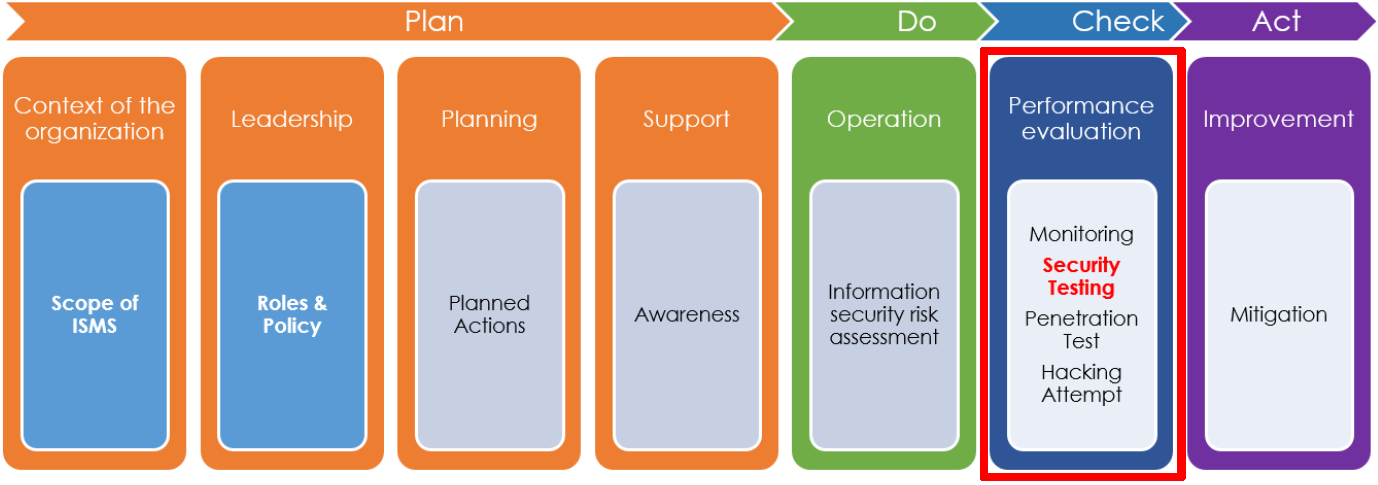
\includegraphics[width=\textwidth]{./img/ISO27001_overview}
	\caption{Stark vereinfachte Sicht [ISO27001:2005]}
\end{figure}

\begin{description}
	\item[Threat] Effekte, \textbf{können nicht} kontrolliert werden (Erdbeben, Stromausfall).
	\item[Risk] Risiko, kann vermindert werden durch verminderung des Einflusses auf das Business.
	\item[Vulnerability] Gefahren, können behandelt werden (Verbesserung der Software, Einschränken von Zugriff).
	\item[Vulnerability Assessment] Das eigentliche Information Security Management: Geschäftsprozesse werden beobachtet, verknüpft mit der Compliance, Budget, Beurteilung und der Bewusstheit der Gefahr.
	\item[Direct Attacks] Angriff direkt auf das Ziel, z.B. durch eine Firewall.
	\item[Indirect Attack] Ein ungeschütztes Gerät, wie z.B. ein privates Notebook, wird angegriffen und über dieses dann dem Angreifer Zugriff auf das restliche System ermöglicht.
	\item[Man-in-the-Middle] Der Angreifer hört den Datenverkehr des Opfers mit und kann diesen auch beeinflussen, erneut versenden oder verändern.
	\item[Privilege Escalation] Es wird versucht, mehr Berechtigungen zu erhalten, wie z.B. ausführen eines Skripts als Root, ohne die Kennwörter zu besitzen.
	\item[Social Engineering] Umgehen von technischen Einrichtungen zum Schutz vor Angriffen über menschliches Fehlverhalten und gezielte Manipulation des Menschen.
	\item[Backdoor] Teil einer Software/Hardware, unter Umgehung der normalen Zugriffssicherung Zugang zu geschützten Daten zu erlangen.
\end{description}

\subsubsection{Symantec Internet Security Threat Report}
Symantec veröffentlich seit nunmehr 20 Jahren jeden Frühling ihren Internet Security Threat Report, der jeweils die wichtigsten Bedrohungen des vergangenen Kalenderjahres analysiert und im Vergleich zu vorhergehenden Jahren die aktuellen Trends aufzeigt.

Folgende Punkte werden hauptsächlich thematisiert:
\begin{easylist}[itemize]
	& Mobile Devices
	& Internet of Things
	& Web Threats
	& Social Media, Scams and Email Threats
	& Targeted Attacks
	& Data Breaches
	& Cloud Infrastructure
	& Best Practice Guidelines
\end{easylist}